\section{包设计}
\subsection{整体架构设计}
本系统为了能更加有效地进行整合、生产宏观模型,就需要对系统中的类进行分组,以下是本系统中的包设计。
\begin{figure}[!htbp]
	\centering
	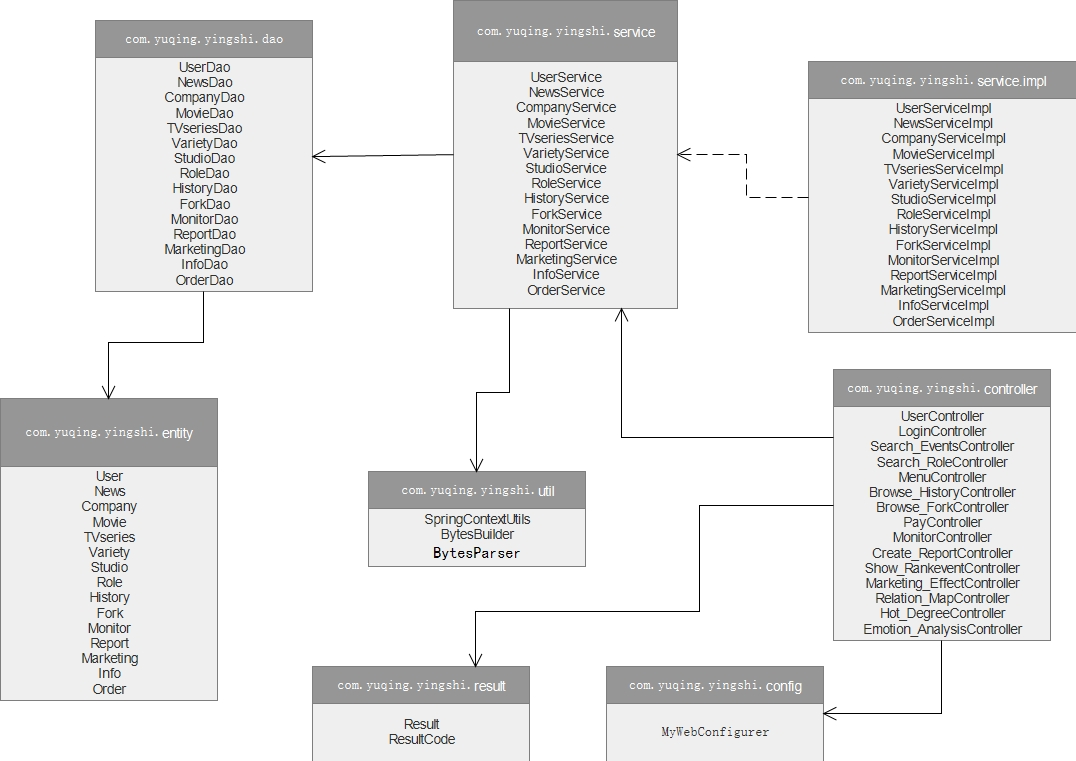
\includegraphics[scale=0.4]{image/o2.png}
	\caption{舆情系统包的设计图}
\end{figure}

\subsection{包的设计说明}
下表为服务器的包设计表
\begin{tabular}{c c|} 
包名 & 
\multicolumn{2}{c}{设计说明} \\ 
\hline 
com.yuqing.yingshi.service & 该包主要存放了高层调用Dao的接口\\
com.yuqing.yingshi.controller & 改包主要存放了业务逻辑相关类,依赖于com.yuqing.yingshi.service,调用Service以完成业务逻辑\\
com.yuqing.yingshi.result& 该包存放了服务器与web端交互时返回的结果对应编码\\
com.yuqing.yingshi.dao&主要负责数据访问,该包中的类封装了对数据库的访问(只包含最原子的数据操作),供高层调用,依赖于com.yuqing.yingshi.entity\\
com.yuqing.yingshi.config& 存放了与前端web网页交互的相关配置\\
com.yuqing.yingshi.entity&该包主要存放数据库表中所对应的实体类\\
com.yuqing.yingshi.service.impl&该包存放了service包中定义的接口的具体实现\\
com.yuqing.yingshi.util&存放了项目相关工具类\\
\end{tabular}

\section{类设计}
本小结以包为单位,对每个包所含有的类及类与类间的调用关系进行说明。
\begin{tabular}{|c|c|} 
\hline 
\multicolumn{2}{|c|}{com.yuqing.yingshi.dao相关类} \\ 
\hline 
UserDao&封装与User实体类相关的数据访问方法\\
NewsDao&封装与News实体类相关的数据访问方法\\
CompanyDao&封装与Company实体类相关的数据访问方法\\
MovieDao&封装与Movie实体类相关的数据访问方法\\
TVseriesDao&封装与TVseries实体类相关的数据访问方法\\
VarietyDao&封装与Variety实体类相关的数据访问方法\\
StudioDao&封装与Studio实体类相关的数据访问方法\\
RoleDao&封装与Role实体类相关的数据访问方法\\
HistoryDao&封装与History实体类相关的数据访问方法\\
ForkDao&封装与Fork实体类相关的数据访问方法\\
MonitorDao&封装与Monitor实体类相关的数据访问方法\\
ReportDao&封装与Report实体类相关的数据访问方法\\
MarketingDao&封装与Marketing实体类相关的数据访问方法\\
InfoDao&封装与Info实体类相关的数据访问方法\\
OrderDao &封装与Order实体类相关的数据访问方法\\
\hline 
\end{tabular}


\begin{tabular}{|c|c|} 
\hline 
\multicolumn{2}{|c|}{com.yuqing.yingshi.entity相关类} \\ 
\hline 
User &用户个人信息的实体类\\
News &新闻信息的实体类\\
Company &公司信息的实体类\\
Movie&电影信息的实体类\\
TVseries&影视剧信息的实体类\\
Variety&综艺信息的实体类\\
Studio&工作室信息的实体类\\
Role&演员/歌手等明星信息的实体类\\
History&历史记录的实体类\\
Fork&收藏记录的实体类\\
Monitor&监控预警项的实体类\\
Report&报告的实体类\\
Marketing&营销效果的实体类\\
Info &单条博文/帖子信息的实体类\\
Order &用户订单的实体类\\
\hline 
\end{tabular}



\begin{tabular}{|c|c|} 
\hline 
\multicolumn{2}{|c|}{com.yuqing.yingshi.service相关类} \\ 
\hline 
UserService&定义了与User实体类相关的业务逻辑接口\\
NewsService&定义了与News实体类相关的业务逻辑接口\\
CompanyService&定义了与Company实体类相关的业务逻辑接口\\
MovieService&定义了与Movie实体类相关的业务逻辑接口\\
TVseriesService&定义了与TVseries实体类相关的业务逻辑接口\\
VarietyService&定义了与Variety实体类相关的业务逻辑接口\\
StudioService&定义了与Studio实体类相关的业务逻辑接口\\
RoleService&定义了与Role实体类相关的业务逻辑接口\\
HistoryService&定义了与History实体类相关的业务逻辑接口\\
ForkService&定义了与Fork实体类相关的业务逻辑接口\\
MonitorService&定义了与Monitor实体类相关的业务逻辑接口\\
ReportService&定义了与Report实体类相关的业务逻辑接口\\
MarketingService&定义了与Marketing实体类相关的业务逻辑接口\\
InfoService&定义了与Info实体类相关的业务逻辑接口\\
OrderService&定义了与Order实体类相关的业务逻辑接口\\
\hline 
\end{tabular}

\begin{tabular}{|c|c|} 
\hline 
\multicolumn{2}{|c|}{com.yuqing.yingshi. controller相关类} \\ 
\hline 
UserControlle&定义了响应用户相关界面不同点击事件的方法,根据事件的不同调用 UserService的相应方法实现功能,以json格式返回。\\
LoginController&定义了登陆注册界面不同点击事件的方法,根据事件的不同调用 UserService的相应方法实现功能,以json格式返回。\\
Search_EventsController&定义了搜索热门影视事件/影视作品相关界面不同点击事件的方法,根据事件的不同调用 NewsService、MovieService、TVseriesService、VarietyService的相应方法实现功能,以json格式返回。\\
Search_RoleController&定义了搜索明星/公司/工作室相关界面不同点击事件的方法,根据事件的不同调用 RoleService、CompanyService、StudioService的相应方法实现功能,以json格式返回。\\
MenuController&定义了展示影视事件/明星/影视作品菜单相关界面不同点击事件的方法,根据事件的不同调用 RoleService、CompanyService、StudioService、NewsService、MovieService、TVseriesService、VarietyService的相应方法实现功能,以json格式返回。\\
Browse_HistoryController&定义了浏览历史记录相关界面不同点击事件的方法,根据事件的不同调用 HistoryService的相应方法实现功能,以json格式返回。\\
Browse_ForkController&定义了浏览收藏记录相关界面不同点击事件的方法,根据事件的不同调用 ForkService的相应方法实现功能,以json格式返回。\\
PayController&定义了会员支付相关界面不同点击事件的方法,根据事件的不同调用 PayService的相应方法实现功能,以json格式返回。\\
MonitorController&定义了监控预警相关界面不同点击事件的方法,根据事件的不同调用 MonitorService的相应方法实现功能,以json格式返回。\\
Create_ReportController&定义了生成报告相关界面不同点击事件的方法,根据事件的不同调用 ReportService的相应方法实现功能,以json格式返回。\\
Show_RankeventController&定义了热门事件排行榜相关界面不同点击事件的方法,根据事件的不同调用 NewsService的相应方法实现功能,以json格式返回。\\
Marketing_EffectController&定义了营销效果分析与追踪相关界面不同点击事件的方法,根据事件的不同调用 NewsService的相应方法实现功能,以json格式返回。\\
Relation_MapController&定义了明星关系图谱相关界面不同点击事件的方法,根据事件的不同调用 RoleService的相应方法实现功能,以json格式返回。\\
Hot_DegreeController&定义了分析事件热度相关的功能与方法,根据事件的不同调用 RoleService、CompanyService、StudioService、NewsService、MovieService、TVseriesService、VarietyService的相应方法实现功能,以json格式返回。\\
Emotion_AnalysisController&定义了情感分析相关的功能与方法,根据事件的不同调用RoleService、CompanyService、StudioService、NewsService、MovieService、TVseriesService、VarietyService的相应方法实现功能,以json格式返回。\\
\hline 
\end{tabular}

\begin{tabular}{|c|c|} 
\hline 
\multicolumn{2}{|c|}{com.yuqing.yingshi.config相关类} \\ 
\hline 
MyWebConfigurer& 定义了与前端web页面交互的相关配置\\
\hline 
\end{tabular}

\begin{tabular}{|c|c|} 
\hline 
\multicolumn{2}{|c|}{com.yuqing.yingshi.util相关类} \\ 
\hline 
SpringContextUtils&获取spring容器bean对象工具类\\
BytesBuilder&字节构造器\\
BytesParser&字节处理器\\
\hline 
\end{tabular}

\begin{tabular}{|c|c|} 
\hline 
\multicolumn{2}{|c|}{com.yuqing.yingshi.result相关类} \\ 
\hline 
Result&结果返回形式定义\\
ResultCode&定义返回结果编码\\
\hline 
\end{tabular}
\section{接口设计}
\subsection{外部接口设计}
外部接口是各模块间进行交互访问以及web访问系统时的外部接口,某一模块的具体功能则由内部接口设计实现。
\begin{figure}[!htbp]
	\centering
	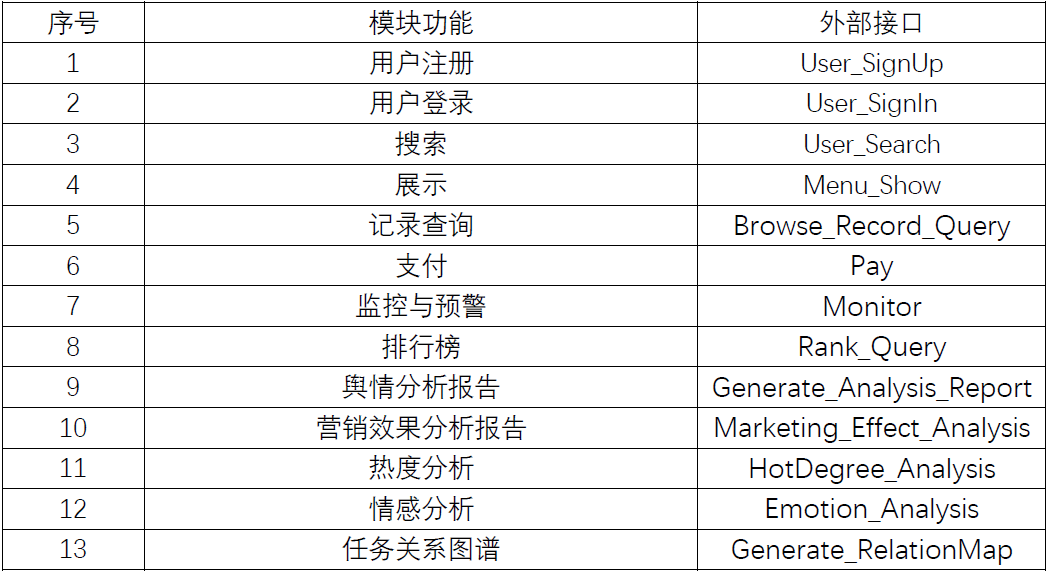
\includegraphics[scale=0.4]{image/m1.png}
	\caption{外部接口设计}
\end{figure}
\subsection{内部接口设计}
\subsubsection{注册登录模块}
\begin{figure}[!htbp]
	\centering
	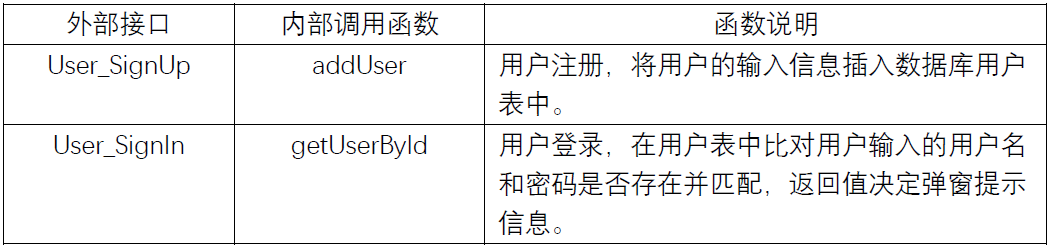
\includegraphics[scale=0.4]{image/m2.png}
	\caption{注册登录模块}
\end{figure}
\subsubsection{搜索模块}
\begin{figure}[!htbp]
	\centering
	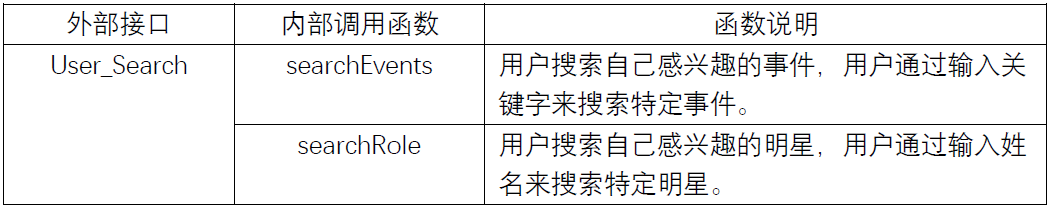
\includegraphics[scale=0.4]{image/m3.png}
	\caption{搜索模块}
\end{figure}
\subsubsection{展示模块}
\begin{figure}[!htbp]
	\centering
	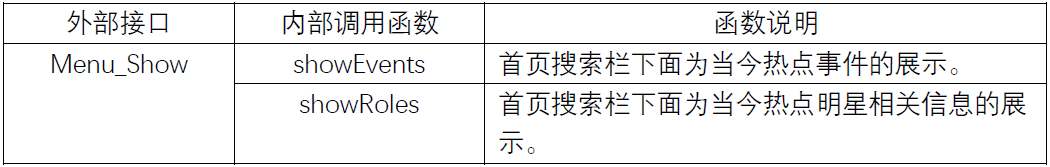
\includegraphics[scale=0.4]{image/m4.png}
	\caption{展示模块}
\end{figure}
\subsubsection{记录查询模块}
\begin{figure}[!htbp]
	\centering
	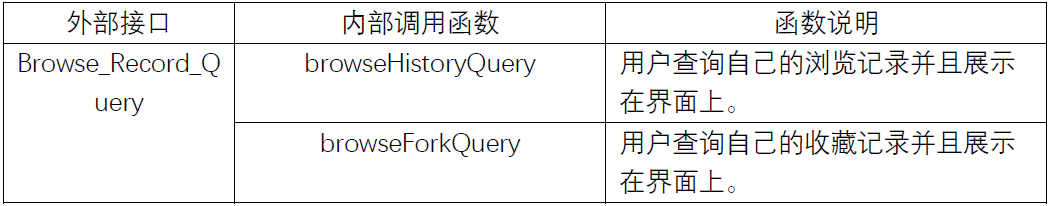
\includegraphics[scale=0.4]{image/m5.png}
	\caption{记录查询模块}
\end{figure}
\subsubsection{支付模块}
\begin{figure}[!htbp]
	\centering
	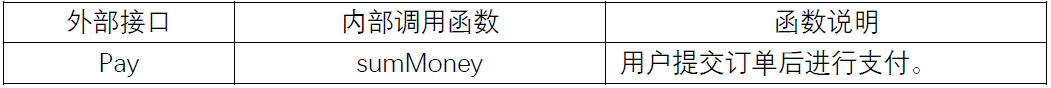
\includegraphics[scale=0.4]{image/m6.png}
	\caption{支付模块}
\end{figure}
\subsubsection{监控与预警模块}
\begin{figure}[!htbp]
	\centering
	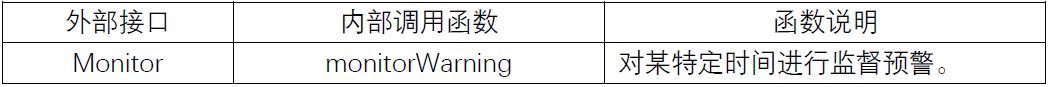
\includegraphics[scale=0.4]{image/m7.png}
	\caption{监控与预警模块}
\end{figure}
\subsubsection{排行榜模块}
\begin{figure}[!htbp]
	\centering
	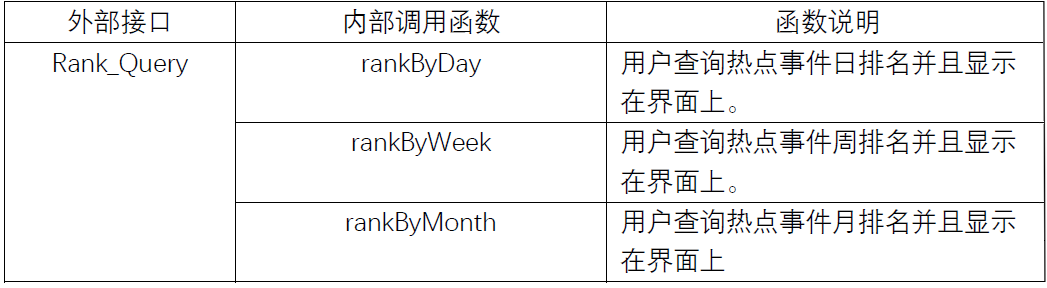
\includegraphics[scale=0.4]{image/m8.png}
	\caption{排行榜模块}
\end{figure}
\subsubsection{分析模块}
\begin{figure}[!htbp]
	\centering
	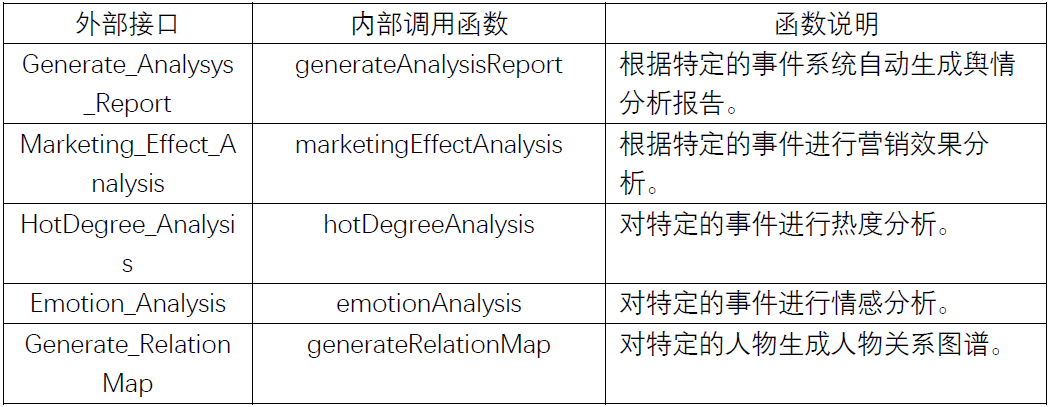
\includegraphics[scale=0.4]{image/m9.png}
	\caption{分析模块}
\end{figure}
